




\begin{lemma}\label{l:consistencyEndGBS}



Let $\alpha_{Mi}$ and $\beta_{Mi}$ be the parameters for each of the $4$ failure models Mi as reported in Table \ref{t:parameters} and used by the algorithm in Fig. \ref{fig:server}-\ref{fig:client}.
Let $n > \alpha_{Mi} f$ for each failure model Mi considered. 
At the end of each round, at least $n-f$ correct servers store the same value $v$ in their $value_i$ local variable.
\end{lemma}

\begin{proofL}
Each non-faulty server updates its $value_i$ local variable at the end of each round $r$ (i) in line  \ref{s21} i.e., if there exists at least a pair in the $current\_writes_i$ local variable, or (ii) in line  \ref{s23} i.e., $current\_writes_i$ is empty and there exist at least $n-\beta f$ same values in $echo\_vals_i$.


First we prove that one of the two cases always happens and then we prove that the number of non-faulty servers storing the same values $v$ is $n-f$.
The $current\_writes_i$ local variable is initialized by any non-faulty server $s_i$ to $\emptyset$ at the beginning of each round $r$ (cfr. line \ref{s2}) and it is updated when a {\sc write}$()$ message is received by $s_i$\footnote{Recall that such {\sc write}$()$ message is sent by the writer client in the send phase of the first round starting after the ${\sf write}()$ invocation and it is delivered by any non-faulty server in the same round.}.
Thus, case (i) corresponds to a scenario where at least a ${\sf write}()$ operation is executed in round $r$ and case (ii) corresponds to a scenario where no ${\sf write}()$ is running.

\begin{itemize}
\item {\bf Case (i):} $\mathbf{current\_writes_i \neq \emptyset.}$ In this case the claim simply follows by considering that (i) writer clients broadcast a {\sc write}$(v, j)$ message in the send phase of round $r$, (ii) clients are correct so the same set of values is delivered to all servers that will apply a deterministic function to select the value $v$ and (iii) at most $f$ servers are faulty and may skip the update of their $value_i$ variable.\\

\item {\bf Case (ii):} $\mathbf{current\_writes_i = \emptyset}$ {\bf and line \ref{s22} is true.} In this case, the $value_i$ variable is updated according to the values stored in $echo\_vals_i$. Such variable is emptied by every non-faulty process at the beginning of each round (cfr. line \ref{s1}) and is filled in when an {\sc echo}$()$ message is delivered.
Such message is sent at least by any server, believing it is correct, at the beginning of each round.
Let $r'$ be the round in which the last ${\sf write}(v)$ operation terminated. Note that, due to above hypothesis, a ${\sf write}()$ operation always exists as we assume a fictional write happening instantaneously at round $r_0$. Without loss of generality, let us consider the round $r=r'+1$.
Due to case (i), at the end of $r'$, at least $n-f$ non-faulty servers store the same value $v$ in their local variable $value_i$.
Thus, at the beginning of $r'+1$, at least $n-f-x$ correct servers will send an {\sc echo}$(v, j)$ message, where $x$ is the number of non-faulty processes that become faulty while passing from $r'$ to $r$ (i.e. $x=f$ for all the models but Burhman's one where $x=0$ as faulty processes move during the send phase and not at the beginning of the round).
It follows that the condition in line \ref{s22} is verified if and only if $n-f-x \ge n-\beta f$ that is true in any model.
Therefore, considering that at the end of round $r$ non-faulty servers are exactly $n-f$, we have that $n-f$ processes will execute this update.
Iterating the reasoning for any $r$ the claim follows.

\end{itemize}


\renewcommand{\toto}{l:consistencyEndGBS}
\end{proofL}














\begin{lemma}\label{l:writeTermination}
Let us consider the algorithm in Fig. \ref{fig:server}-\ref{fig:client}. If a correct client invokes a {\sf write}$()$ operation, it eventually returns from that operation. 
\end{lemma}

\begin{proofL}
	The proof simply follows by considering that, for a ${\sf write}()$ operation invoked at some round $r$,  the ${\sf write\_confirmation}$ is generated by the client at the end of the same round just checking the value of the variables initialized at the beginning of $r$.
\renewcommand{\toto}{l:writeTermination}
\end{proofL}
	
\begin{lemma}\label{l:readTermination}


Let $\alpha_{Mi}$ and $\beta_{Mi}$ be the parameters for each of the $4$ failure models Mi as reported in Table \ref{t:parameters} and used by the algorithm in Fig. \ref{fig:server}-\ref{fig:client}.
Let $n > \alpha_{Mi} f$ for each failure model Mi considered. 
If a correct client invokes a ${\sf read}()$ operation, it eventually returns from that operation. 
\end{lemma}

\begin{proofL}
Let $c_j$ be a client invoking a ${\sf read}()$ operation at some time $t$. 
When this happens, $c_j$ flags that a ${\sf read}()$ operation is starting and prepares a {\sc read}$()$ message to send at the beginning of the next {\em send} phase at round $r$. 
When $c_j$ sends such {\sc read}$()$ message, it updates its $op\_start_j$ variable to $r$ and it returns from the ${\sf read}()$ operation at round $r+1$ if and only if it has at least $n-\beta f$ occurrences of the same value in the $replies_j$ set.
Such $replies_j$ is initially empty (it has been emptied at the end of the previous ${\sf read}()$ operation) and it is filled in when $c_j$ receives a {\sc reply}$()$ message (line \ref{c11}) that is sent at least by non-faulty servers when they receive a {\sc read}$()$ message.

In particular, the {\sc read}$()$ message sent by $c_j$ will be delivered by servers during the receiving phase of round $r$. When this happens, any non-faulty server will execute line \ref{s18} in Figure \ref{fig:server} and will store the identifier of $c_j$ in order to send a reply at the beginning of the next round $r+1$. 
Due to Lemma \ref{l:consistencyEndGBS}, at the end of round $r$, at least $n-f$ non-faulty servers will store the same value $v$.
Let us note that, during the send phase of round $r+1$, $x$ of such servers may become faulty.
Thus, $c_j$ will find a value satisfying the condition in line \ref{c21} if and only if $n-f-x \ge n-\beta f$.
Considering that $x\le f$ for all models but Burhman's one where $x=0$, we have that the condition is always true and the claim follows.


	
\renewcommand{\toto}{l:readTermination}
\end{proofL}

\begin{theorem}[Termination]\label{t:termination}
	If a correct client invokes an operation, it eventually returns from that operation. 
\end{theorem}

\begin{proofT}
	It follows direclty from Lemma \ref{l:writeTermination} and Lemma \ref{l:readTermination}.
	\renewcommand{\toto}{t:termination}
\end{proofT}

\begin{theorem}[Validity]\label{t:validity}
Let $\alpha_{Mi}$ and $\beta_{Mi}$ be the parameters for each of the $4$ failure models Mi as reported in Table \ref{t:parameters} and used by the algorithm in Fig. \ref{fig:server}-\ref{fig:client}.
Let $n > \alpha_{Mi} f$ for each failure model, Mi, considered. 
Any ${\sf read}()$ operation returns the last value written before its invocation, or a value written by a concurrent ${\sf write}()$ operation. 
\end{theorem}

\begin{proofT}
Without loss of generality, let us consider the first ${\sf write}(v)$ operation $op_W$ and the first ${\sf read}()$ operation $op_R$. 
Three cases may happen: (i) $op_R \prec op_W$, (ii) $op_W \prec op_R$ and (iii) $op_W ~|| ~op_R$.
Let us note that $op_r$ spans over two rounds: in the first one it sends the {\sc read}$()$ message and in the second one it collects replies.

	\begin{itemize}
		\item {\bf Case (i):} $\mathbf{op_R \prec op_W}$. This case follows directly from Lemma \ref{l:consistencyEndGBS} considering that (i) at the end of the first round of $op_r$ (i.e., $r_1$) at least $n-f$ correct processes have the same initial value $v=\bot$, (ii) while moving to the second round of $op_R$, at most $x$ processes can get faulty (with $x\le f$ for models M1-M3 and $x=0$ for M4), (iii) $n-f-x \ge n- \beta_{Mi}f$ (i.e. $\beta_{Mi}f \ge f+x$) for each model (i.e. there will always be enough replies from correct servers to select a value) and (iv) $n- \beta_{Mi}f > f$ (i.e. $(\alpha_{Mi}-\beta_{Mi})f +1 > f$) for each model.
It follows that faulty processes cannot force the client to select a wrong value.\\
		
		\item  {\bf Case (ii):} $\mathbf{op_W \prec op_R}$. Let $r$ be the round at which $op_W$ terminates and let $r+1$ be the round at which $op_R$ is invoked.
		
Due to Lemma \ref{l:consistencyEndGBS}, at round $r+2$ there are enough occurrences (at least $n-\beta f$) of the last written value $v$. So, applying the same reasoning of case (i) the claim follows.\\	
		
		\item {\bf Case (iii):} $\mathbf{op_W ~|| ~op_R}$. Let us note that a ${\sf read}()$ operation spans two rounds, i.e., the round of the request $r_{req}$ and the round of the reply $r_{reply}$. So, let us consider them separately.
		
		\begin{itemize}
			\item {\bf Case (iii-a):} $op_W$ is concurrent with $op_R$ during $r_{req}$. In that case the value $v$ is delivered to correct server at the end of $r_{req}$. Due to Lemma \ref{l:consistencyEndGBS}, at the end of $r_{req}$ at least $n-f$ correct servers store the new written value $v$, we fall down into case (ii) and the claim follows.\\
\item {\bf Case (iii-b):} $op_W$ is concurrent with $op_R$ during $r_{replay}$. Since, in every round, the send phase is executed before the receive phase, it follows that at least all the correct servers will reply with the value written before the invocation of the ${\sf write}()$ operation, we fall down into case (i) and the claim follows.
\end{itemize}	
	\end{itemize}
	
\renewcommand{\toto}{t:validity}
\end{proofT}

\begin{theorem}[Ordering]\label{t:ordering} There exists a total order $S$ of ${\sf read}()$ and ${\sf write}()$ operations such (i) if $op \prec op'$ then $op$ appears before $op'$ in $S$ and (ii) any ${\sf read}()$ operation returns the value $v$ written by the last ${\sf write}()$ preceding it in $S$.
\end{theorem}

\begin{proofL}
	Consider two ${\sf read}()$ operations, $op_{R1}$ and $op_{R2}$ returning respectively $v_1$ and $v_2$ (with $v_1 \neq v_2$) such that $op_{R1} \prec op_{R2}$.
	Note that if $op_{R1}$ returns $v_1$, it follows that there exists a ${\sf write}(v_1)$ operation,  $op_{W(v_1)}$ concurrent or preceding it in $S$. 
	Suppose by contradiction that $op_{W(v_2)} \prec op_{W(v_1)}$. Recall that each ${\sf read}()$ operation spans over two rounds and call the first $r_{req}$ and the second $r_{reply}$.
Since $op_{R1}$ returns $v_1$ this means that $v_1$ has been stored by servers at latest during $r_{req}$ of $op_{R1}$; let us call it $r_{R1req}$. The same holds for $op_{R2}$: $v_2$ has been written at most during $r_{R2req}$ of $op_{R2}$. 
	Since $op_{R2}$ follows $op_{R1}$ then $r_{R1req}<r_{R2req}$. However, which is a contradiction to respect the assumption of $r_{v1}>r_{v2}$ (a general scenario is depicted in Fig.\ref{fig:scenarioOrdering}).
	\renewcommand{\toto}{t:ordering}
\end{proofL}


\begin{figure}
	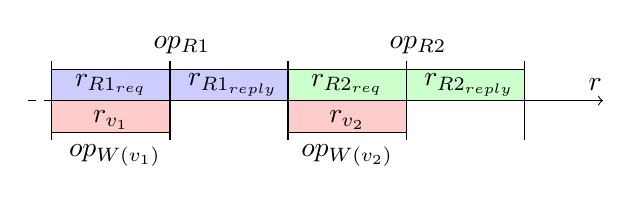
\begin{tikzpicture}
	
	\draw[->] (-.3, 0) -- (-.2,0) (-.1,0) -- (7,0);\node[] at (6.9,.2) {$r$};
	
	\filldraw[fill=blue!20!white, draw=black] (0,0) rectangle (3,.4);
	\filldraw[fill=red!20!white, draw=black] (0,0) rectangle (1.5,-.4);
	\draw (0,-.5) -- (0,.5) (1.5,-.5) -- (1.5,.5);
	\draw[thick] (3,-.5) -- (3,.5);
	\filldraw[fill=green!20!white, draw=black] (3,0) rectangle (6,.4);
	\filldraw[fill=red!20!white, draw=black] (3,0) rectangle (4.5,-.4);
	\draw  (4.5,-.5) -- (4.5,.5);
	\draw  (6,-.5) -- (6,.5);
	
	\node[] at (.75,-.25) {$r_{v_1}$}; \node[] at (.75,.2) {$r_{R1_{req}}$}; \node[] at (2.3,.2) {$r_{R1_{reply}}$};
	\node[] at (1.65,.7) {$op_{R1}$}; \node[] at (.8,-.7) {$op_{W(v_1)}$};
	\node[] at (3.75,-.25) {$r_{v_2}$}; \node[] at (3.75,.2) {$r_{R2_{req}}$}; \node[] at (5.3,.2) {$r_{R2_{reply}}$};
	\node[] at (4.65,.7) {$op_{R2}$}; \node[] at (3.75,-.7) {$op_{W(v_2)}$};
	
	\end{tikzpicture}
	\caption{A general scenario which show how two subsequent ${\sc read}()$ operations $op_{R1}$ and $op_{R2}$ can not return respectively $v_1$ and $v_2$ if $v_2$ has been written before $v_1$.}
	\label{fig:scenarioOrdering}
\end{figure}

\begin{theorem}\label{th:Garay}
	Let $\mathcal{A}_{Areg}$ be the algorithm in Fig. \ref{fig:server}-\ref{fig:client} and let $n > \alpha f$.
	If $\alpha = 3$ and $\beta = 2$ then $\mathcal{A}_{Areg}$ implements a MWMR Atomic register in the Garay's model.
	
\end{theorem}

\begin{proofT}
	It follows directly from Theorem \ref{t:termination}, \ref{t:validity} and \ref{t:ordering}.
	\renewcommand{\toto}{th:Garay}	
\end{proofT}

\begin{theorem}\label{th:Bonnet}
Let $\mathcal{A}_{Areg}$ be the algorithm in Fig. \ref{fig:server}-\ref{fig:client} and let $n > \alpha f$.
	If $\alpha = 4$ and $\beta = 2$ then $\mathcal{A}_{Areg}$ implements a MWMR Atomic register in the Bonnet's model.
\end{theorem}

\begin{proofT}
	It follows directly from Theorem \ref{t:termination}, \ref{t:validity} and \ref{t:ordering}.
	\renewcommand{\toto}{th:Bonnet}	
\end{proofT}

\begin{theorem}\label{th:Sasaki}
Let $\mathcal{A}_{Areg}$ be the algorithm in Fig. \ref{fig:server}-\ref{fig:client} and let $n > \alpha f$.
	If $\alpha = 4$ and $\beta = 2$ then $\mathcal{A}_{Areg}$ implements a MWMR Atomic register in the Sasaki's model.
\end{theorem}

\begin{proofT}
	It follows directly from Theorem \ref{t:termination}, \ref{t:validity} and \ref{t:ordering}.
	\renewcommand{\toto}{th:Sasaki}	
\end{proofT}

\begin{theorem}\label{th:Burhman}
Let $\mathcal{A}_{Areg}$ be the algorithm in Fig. \ref{fig:server}-\ref{fig:client} and let $n > \alpha f$.
	If $\alpha = 2$ and $\beta = 1$ then $\mathcal{A}_{Areg}$ implements a MWMR Atomic register in the Burhman's model.\end{theorem}

\begin{proofT}
	It follows directly from Theorem \ref{t:termination}, \ref{t:validity} and \ref{t:ordering}.
	\renewcommand{\toto}{th:Burhman}	
\end{proofT}

